\chapter{Pesquisa}
\label{char:pesquisa}
O questionário de \textit{feedback} de utilização do simulador foi disponibilizado através da utilização do \textit{Google Forms} através do link \textit{https://forms.gle/f1DAgWvTyM2uJyLt9}.

\begin{figure}[H]
    \centering
    \caption{Inicio do questionário}
    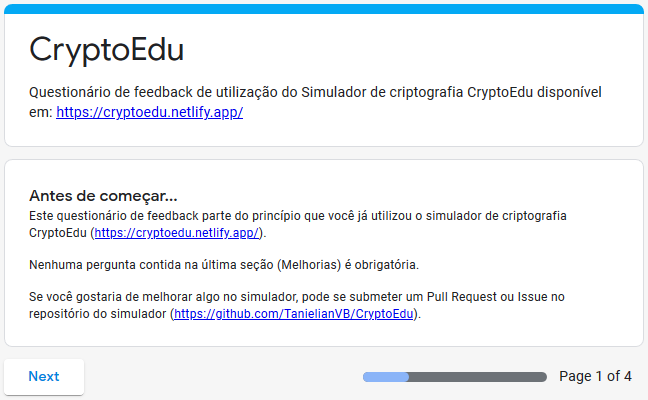
\includegraphics[width=0.75\linewidth]{Questionario/QI.png}
\end{figure}

Antes de apresentar as questões para o usuário é apresentado essa tela de apresentação do questionário.

\section{Perguntas}
O questionário é composto de 6 perguntas, sendo 4 obrigatórias e 2 opcionais, que serão descritas à seguir.

Um fator que foi levado em consideração ao desenvolver o  questionário é a dificuldade de adquirir respostas dos usuários do simulador. Tanto por esse motivo quando para facilitar a análise dos resultados se optou por se utilizar somente de perguntas de múltipla escolha.

\subsection{Enquadramento do usuário}

\begin{figure}[H]
    \centering
    \caption{Enquadramento do usuário}
    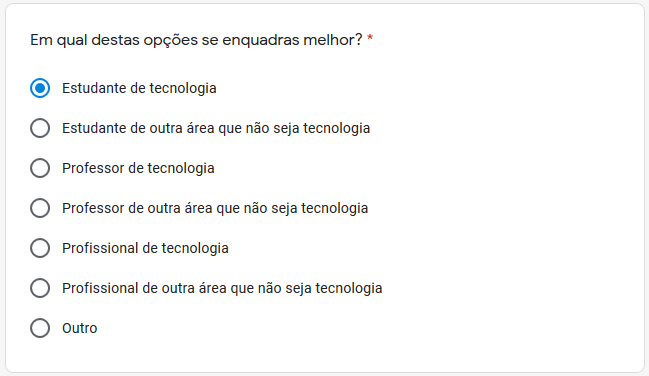
\includegraphics[width=0.75\linewidth]{Questionario/Q1.png}
\end{figure}

Esta pergunta tem como objetivo ter uma \textit{baseline} do tipo de usuário que está respondendo o questionário e dessa forma ser capaz de obter uma curva de crescimento por 'perfil'.

\subsection{Conhecimento antes e depois da utilização do simulador}
Com as próximas 2 perguntas tem-se como objetivo ser capaz de mensurar o crescimento do nível de conhecimento do usuário nos processos presentes no algorítimo S-DES. O escopo das perguntas envolve os processos (permutação, rotação, substituição, xor e troca) presentes no algorítimo ao invés das etapas (P10, LS-1, P8, LS-2, IP, etc...) pois munido do conhecimento dos processos todas as etapas podem ser facilmente reproduzidas.

\begin{figure}[H]
    \centering
    \caption{Conhecimento antes da utilização do simulador}
    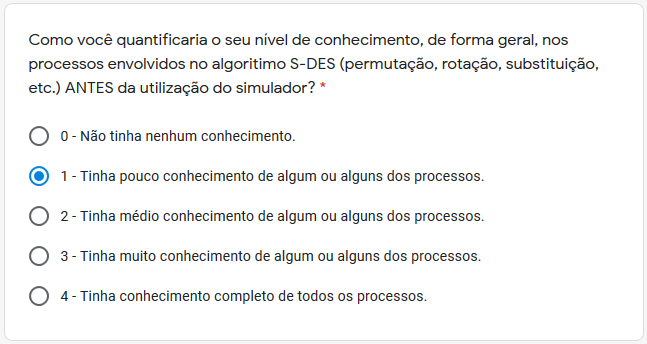
\includegraphics[width=0.75\linewidth]{Questionario/Q2.png}
\end{figure}

Para mensurar esse crescimento é questionado primeiramente como o usuário quantificaria o nível de conhecimento, de maneira geral, que ele possui nos processos presentes no algorítimo antes da utilização do simulador. Buscando obter o ponto de partida da curva de crescimento.

\begin{figure}[H]
    \centering
    \caption{Conhecimento depois da utilização do simulador}
    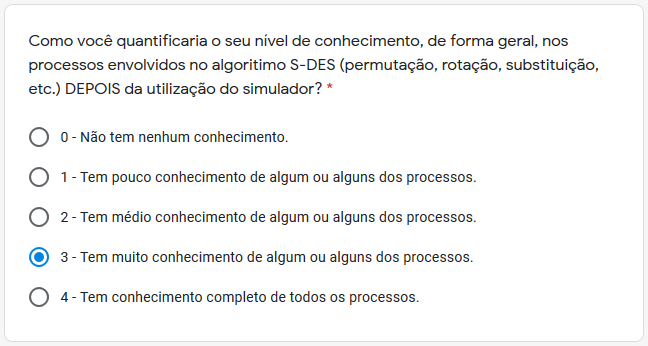
\includegraphics[width=0.75\linewidth]{Questionario/Q3.png}
\end{figure}

A próxima pergunta indaga esse mesmo nível de conhecimento após a utilização do simulador. Buscando obter o ponto de chegada da curva de crescimento.

\subsection{Efetividade do aprendizado}

\begin{figure}[H]
    \centering
    \caption{Efetividade do aprendizado}
    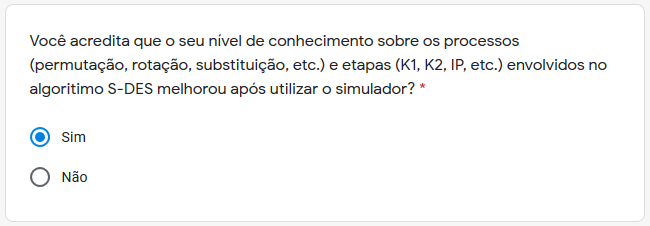
\includegraphics[width=0.75\linewidth]{Questionario/Q4.png}
\end{figure}

Esta pergunta tem como objetivo mensurar, de maneira absoluta, se existiu ganho de conhecimento por parte do usuário.

\subsection{Melhorias no simulador}

Com as próximas 2 perguntas tem-se como objetivo ser capaz de identificar quais etapas explícitas no simulador precisam ser melhoradas. O escopo das perguntas envolve as etapas (P10, LS-1, P8, LS-2, IP, etc...) presentes no algorítimo ao invés dos processos (permutação, rotação, substituição, xor e troca) pois cada descrição e execução é singular àquela determinada etapa.

\begin{figure}[H]
    \centering
    \caption{Melhorias nas descrições das etapas}
    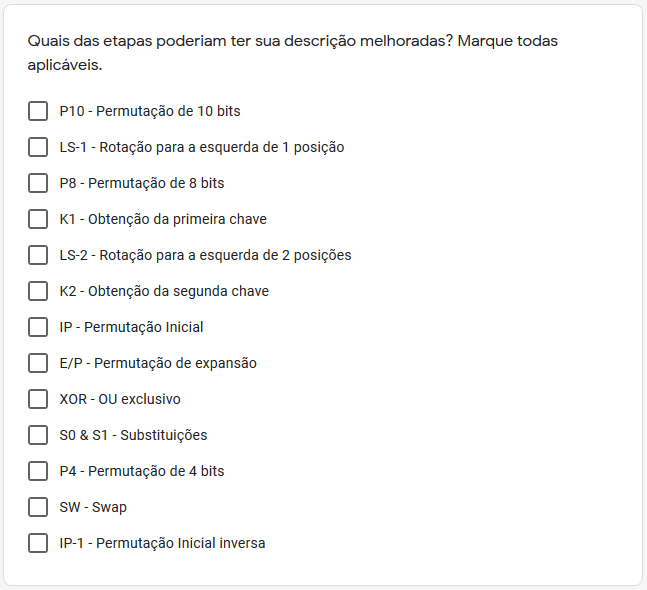
\includegraphics[width=0.7\linewidth]{Questionario/Q5.png}
\end{figure}

A primeira pergunta dessa seção destina-se à identificar quais etapas da execução do algorítimo possuem explicações que podem ser melhoradas, ou seja, não foram suficiente para compreensão completa da etapa pelo usuário.

\begin{figure}[H]
    \centering
    \caption{Melhorias nas execuções das etapas}
    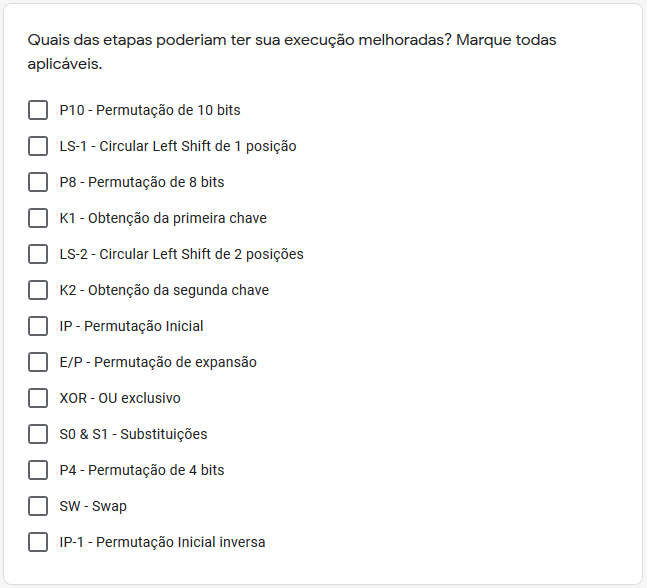
\includegraphics[width=0.7\linewidth]{Questionario/Q6.png}
\end{figure}

A segunda pergunta dessa seção destina-se à identificar quais etapas da execução do algorítimo possuem execuções (passo a passo) que podem ser melhoradas, ou seja, não foram suficiente para compreensão completa do passo a passo da etapa pelo usuário.

\section{Respostas}

O questionário foi submetido à alunos e professores da \acrshort{fbuni} e da \acrshort{unifor}, como também à profissionais das seguintes empresas: Unimake, RCN e Fortes Tecnologia.

\subsection{Enquadramento do usuário}

\begin{figure}[H]
    \centering
    \caption{Enquadramento do usuário}
    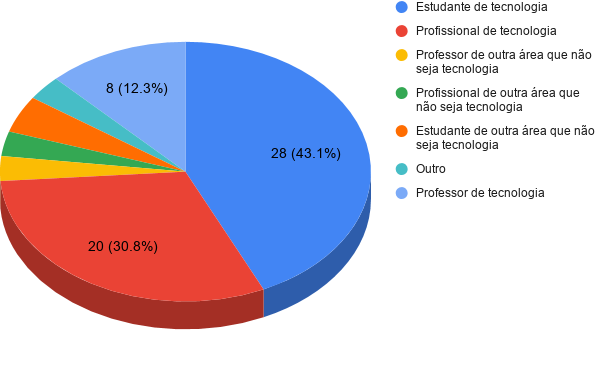
\includegraphics[width=.65\linewidth]{Questionario/CQ1.png}
\end{figure}

Foram obtidas 65 respostas. Sendo 86,2\% da área tecnológica onde 43,1\% são estudantes, 30,8\% profissionais e 12,3\% professores. Embora esse montante não seja o suficiente para um estudo do ponto de vista estatístico, é suficiente para mensurar a efetividade da ferramenta desenvolvida.

\subsection{Conhecimento antes e depois da utilização do simulador}

\begin{figure}[H]
    \centering
    \caption{Conhecimento antes vs. depois da utilização do simulador por enquadramento}
    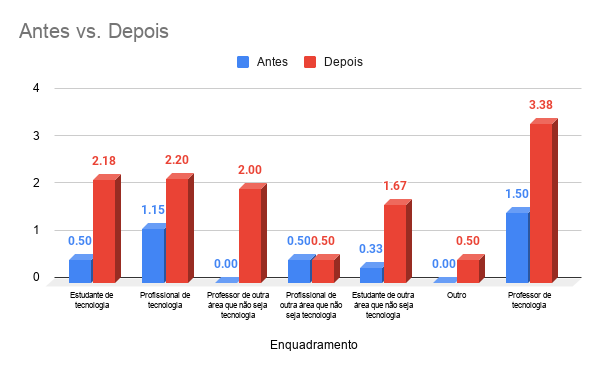
\includegraphics[width=.9\linewidth]{Questionario/CQ2Q3.png}
\end{figure}

Analisando o nível de conhecimento antes e depois para cada enquadramento temos:

\begin{itemize}
    \item Estudantes de tecnologia apresentaram um aumento médio de 1,68 pontos. A média de conhecimento antes era entre \textbf{nenhum} e \textbf{pouco} e após a utilização do simulador passou a ser \textbf{médio} ou superior.
    \item Profissionais de tecnologia apresentaram um aumento médio de 1,05 pontos. A média de conhecimento antes era \textbf{pouco} e após a utilização do simulador passou a ser \textbf{médio} ou superior.
    \item Professores de tecnologia apresentaram um aumento médio de 1,88 pontos. A média de conhecimento antes era entre \textbf{pouco} e \textbf{médio} e após a utilização do simulador passou a ser \textbf{muito} ou superior.
\end{itemize}

Infelizmente, não foram obtidos dados suficientes dos outros enquadramentos que tornasse viável extrair qualquer tipo de conclusão sobre estes.

\subsection{Efetividade do aprendizado}

\begin{figure}[H]
    \centering
    \caption{Efetividade do aprendizado}
    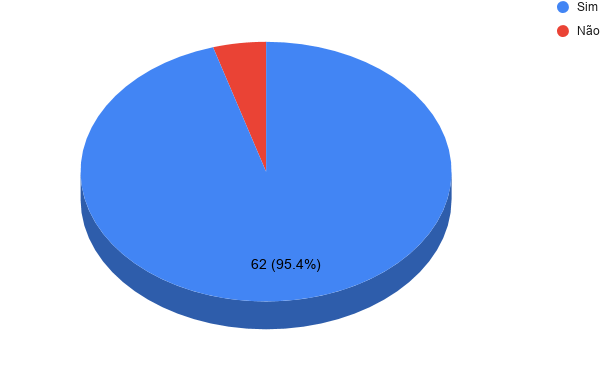
\includegraphics[width=.65\linewidth]{Questionario/CQ4.png}
\end{figure}

95,4\% dos entrevistados consideram que o seu nível de conhecimento sobre os processos e etapas apresentados no simulador melhorou após a utilização do simulador. Um ponto interessante é que mesmo alguns entrevistados que se mensuraram no mesmo nível de conhecimento antes e depois da utilização do simulador ainda assim alegaram ter aprendido com o simulador.

\subsection{Melhorias no simulador}

\begin{figure}[H]
    \centering
    \caption{Melhorias no simulador}
    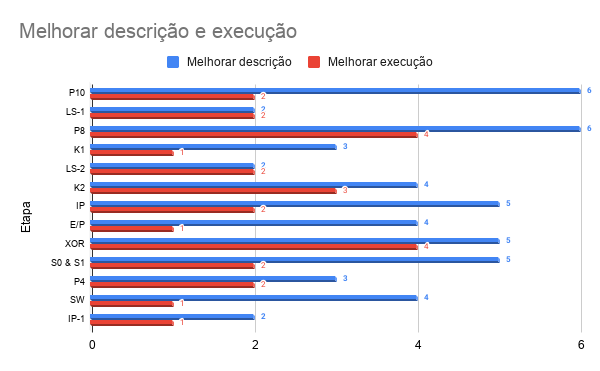
\includegraphics[width=.9\linewidth]{Questionario/CQ5Q6.png}
\end{figure}

Somente 21,53\% dos entrevistados apontaram que algumas etapas poderiam ser melhoradas. Dentre os pontos de melhoria apontados as descrições das permutações e substituição foram os mais indicados como pontos que precisam de melhoria.
